\documentclass[a4paper,11pt,final]{report}

\usepackage[utf8]{inputenc}
\usepackage[english]{babel}
\usepackage[T1]{fontenc}
\usepackage{longtable}
\usepackage{graphicx}
\usepackage{geometry}
\usepackage{hyperref}

\geometry{top=2cm,bottom=2cm,left=2cm,right=2cm}

\title{Lab 4 - Distance Vector Routing}
\author{Romain de Laage (romde686) \& Gyumin Park (gyupa395)\\Group A}
\date{\today}

\begin{document}
\maketitle

\chapter{How distance vector routing works}

Nodes don't have a global knowledge of the network, each node knows the
cost of the link to each of its neighbor and for each neighbor its
distance from each node of the network.

It can build a distance vector by finding the minimum cost for each
neighbor, how many does it cost to go to this neighbor plus what is the
distance from this neighbor to the final node. Then it can build a
optimized routing table. Each update of the distance vector is spread to
the neighbors and on each update received from a neighbor, a node
recompute the minimum cost to go to each node and the routing table.

The algorithm converge to a global optimized network. It is based on
Bellman-Ford equation.

\chapter{Testing}

We tested the solution by making routing table for each node in each
case with a global knowledge of the network (number of node and cost
change enabled or not) and by running the simulator with all the
possible configuration (number of node, poison reverse enabled or not,
link cost change enabled or not). Then we compared the obtained results
with the table we previously made.

So we can check that the algorithm find an optimal solution when it
converge and that poison reverse has an impact on the number of
exchanges between the nodes.

\section{First case, 3 node}

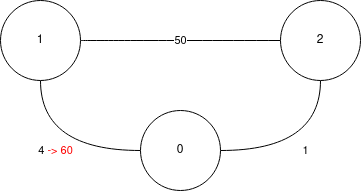
\includegraphics{upload_297bfbc7629abe89b072b536cf2e93ef.png}

In this first case we have a 3 node network. A link cost event can
happen on the link between 1 and 0 from 4 to 60, at time 40.

\subsection{Before link cost change}

The optimized routing table found with a global knowledge of the network
for each node before the link cost change is:

\subsubsection{Node 0}

\begin{tabular}{|c|c|c|c|}
\hline
& 0 & 1 & 2 \\ \hline
Distance & 0 & 4 & 1 \\ \hline
Route & 0 & 1 & 2 \\ \hline
\end{tabular}

\subsubsection{Node 1}

\begin{tabular}{|c|c|c|c|}
\hline
& 0 & 1 & 2 \\ \hline
Distance & 4 & 0 & 5 \\ \hline
Route & 0 & 1 & 0 \\ \hline
\end{tabular}

\subsubsection{Node 2}

\begin{tabular}{|c|c|c|c|}
\hline
& 0 & 1 & 2 \\ \hline
Distance & 1 & 5 & 0 \\ \hline
Route & 0 & 0 & 2 \\ \hline
\end{tabular}

\subsection{After link cost change}

The optimized routing table found with a global knowledge of the network
for each node after the link cost change is:

\subsubsection{Node 0}

\begin{tabular}{|c|c|c|c|}
\hline
& 0 & 1 & 2 \\ \hline
Distance & 0 & 51 & 1 \\ \hline
Route & 0 & 2 & 2 \\ \hline
\end{tabular}

\subsubsection{Node 1}

\begin{tabular}{|c|c|c|c|}
\hline
& 0 & 1 & 2 \\ \hline
Distance & 51 & 0 & 50 \\ \hline
Route & 2 & 1 & 2 \\ \hline
\end{tabular}

\subsubsection{Node 2}

\begin{tabular}{|c|c|c|c|}
\hline
& 0 & 1 & 2 \\ \hline
Distance & 1 & 50 & 0 \\ \hline
Route & 0 & 1 & 2 \\ \hline
\end{tabular}

\section{Second case, 4 node}

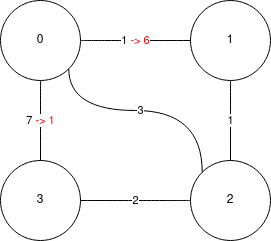
\includegraphics{upload_d59fdf12fdb78f269782a82e8e2dfa44.png}

In this second case we have a 4 node network. A link cost event can
happen on the link between 3 and 0 at time 10,000, a second between 0
and 1 at time 20,000.

\subsection{Before link cost change}

The optimized routing table found with a global knowledge of the network
for each node before the link cost change is:

\subsubsection{Node 0}

\begin{tabular}{|c|c|c|c|c|}
\hline
& 0 & 1 & 2 & 3 \\ \hline
Distance & 0 & 1 & 2 & 4 \\ \hline
Route & 0 & 1 & 1 & 1 \\ \hline
\end{tabular}

\subsubsection{Node 1}

\begin{tabular}{|c|c|c|c|c|}
\hline
& 0 & 1 & 2 & 3 \\ \hline
Distance & 1 & 0 & 1 & 3 \\ \hline
Route & 0 & 1 & 2 & 2 \\ \hline
\end{tabular}

\subsubsection{Node 2}

\begin{tabular}{|c|c|c|c|c|}
\hline
& 0 & 1 & 2 & 3 \\ \hline
Distance & 2 & 1 & 0 & 2 \\ \hline
Route & 1 & 1 & 2 & 3 \\ \hline
\end{tabular}

\subsubsection{Node 3}

\begin{tabular}{|c|c|c|c|c|}
\hline
& 0 & 1 & 2 & 3 \\ \hline
Distance & 4 & 3 & 2 & 0 \\ \hline
Route & 2 & 2 & 2 & 3 \\ \hline
\end{tabular}

\subsection{After first link cost change}

The optimized routing table found with a global knowledge of the network
for each node after the first link cost change is:

\subsubsection{Node 0}

\begin{tabular}{|c|c|c|c|c|}
\hline
& 0 & 1 & 2 & 3 \\ \hline
Distance & 0 & 1 & 2 & 1 \\ \hline
Route & 0 & 1 & 1 & 3 \\ \hline
\end{tabular}

\subsubsection{Node 1}

\begin{tabular}{|c|c|c|c|c|}
\hline
& 0 & 1 & 2 & 3 \\ \hline
Distance & 1 & 0 & 1 & 2 \\ \hline
Route & 0 & 1 & 2 & 0 \\ \hline
\end{tabular}

\subsubsection{Node 2}

\begin{tabular}{|c|c|c|c|c|}
\hline
& 0 & 1 & 2 & 3 \\ \hline
Distance & 2 & 1 & 0 & 2 \\ \hline
Route & 1 & 1 & 2 & 3 \\ \hline
\end{tabular}

\subsubsection{Node 3}

\begin{tabular}{|c|c|c|c|c|}
\hline
& 0 & 1 & 2 & 3 \\ \hline
Distance & 1 & 2 & 2 & 0 \\ \hline
Route & 0 & 0 & 2 & 3 \\ \hline
\end{tabular}

\subsection{After second link cost change}

The optimized routing table found with a global knowledge of the network
for each node after the second link cost change is:

\subsubsection{Node 0}

\begin{tabular}{|c|c|c|c|c|}
\hline
& 0 & 1 & 2 & 3 \\ \hline
Distance & 0 & 4 & 3 & 1 \\ \hline
Route & 0 & 2 & 2 & 3 \\ \hline
\end{tabular}

\subsubsection{Node 1}

\begin{tabular}{|c|c|c|c|c|}
\hline
& 0 & 1 & 2 & 3 \\ \hline
Distance & 4 & 0 & 1 & 3 \\ \hline
Route & 2 & 1 & 2 & 2 \\ \hline
\end{tabular}

\subsubsection{Node 2}

\begin{tabular}{|c|c|c|c|c|}
\hline
& 0 & 1 & 2 & 3 \\ \hline
Distance & 3 & 1 & 0 & 2 \\ \hline
Route & 0 & 1 & 2 & 3 \\ \hline
\end{tabular}

\subsubsection{Node 3}

\begin{tabular}{|c|c|c|c|c|}
\hline
& 0 & 1 & 2 & 3 \\ \hline
Distance & 1 & 3 & 2 & 0 \\ \hline
Route & 0 & 2 & 2 & 3 \\ \hline
\end{tabular}

\section{Third case, 5 node}

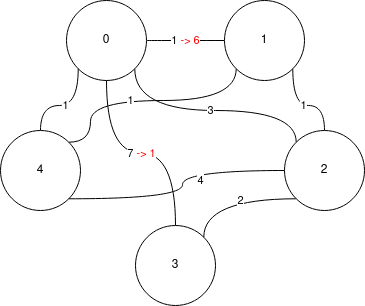
\includegraphics{upload_ce8d2ba305cfd6dabce57e6ab21a2259.png}

In this third case we have a 5 node network. A link cost event can
happen on the link between 3 and 0 at time 10,000, a second between 0
and 1 at time 20,000.

\subsection{Before link cost change}

The optimized routing table found with a global knowledge of the network
for each node before the link cost change is:

\subsubsection{Node 0}

\begin{tabular}{|c|c|c|c|c|c|}
\hline
& 0 & 1 & 2 & 3 & 4 \\ \hline
Distance & 0 & 1 & 2 & 4 & 1 \\ \hline
Route & 0 & 1 & 1 & 1 & 4 \\ \hline
\end{tabular}

\subsubsection{Node 1}

\begin{tabular}{|c|c|c|c|c|c|}
\hline
& 0 & 1 & 2 & 3 & 4 \\ \hline
Distance & 1 & 0 & 1 & 3 & 1 \\ \hline
Route & 0 & 1 & 2 & 2 & 4 \\ \hline
\end{tabular}

\subsubsection{Node 2}

\begin{tabular}{|c|c|c|c|c|c|}
\hline
& 0 & 1 & 2 & 3 & 4 \\ \hline
Distance & 2 & 1 & 0 & 2 & 2 \\ \hline
Route & 1 & 1 & 2 & 3 & 1 \\ \hline
\end{tabular}

\subsubsection{Node 3}

\begin{tabular}{|c|c|c|c|c|c|}
\hline
& 0 & 1 & 2 & 3 & 4 \\ \hline
Distance & 4 & 3 & 2 & 0 & 4 \\ \hline
Route & 2 & 2 & 2 & 3 & 2 \\ \hline
\end{tabular}

\subsubsection{Node 4}

\begin{tabular}{|c|c|c|c|c|c|}
\hline
& 0 & 1 & 2 & 3 & 4 \\ \hline
Distance & 1 & 1 & 2 & 4 & 0 \\ \hline
Route & 0 & 1 & 1 & 1 & 4 \\ \hline
\end{tabular}

\subsection{After first link cost change}

The optimized routing table found with a global knowledge of the network
for each node after the first link cost change is:

\subsubsection{Node 0}

\begin{tabular}{|c|c|c|c|c|c|}
\hline
& 0 & 1 & 2 & 3 & 4 \\ \hline
Distance & 0 & 1 & 2 & 1 & 1 \\ \hline
Route & 0 & 1 & 1 & 3 & 4 \\ \hline
\end{tabular}

\subsubsection{Node 1}

\begin{tabular}{|c|c|c|c|c|c|}
\hline
& 0 & 1 & 2 & 3 & 4 \\ \hline
Distance & 1 & 0 & 1 & 2 & 1 \\ \hline
Route & 0 & 1 & 2 & 0 & 4 \\ \hline
\end{tabular}

\subsubsection{Node 2}

\begin{tabular}{|c|c|c|c|c|c|}
\hline
& 0 & 1 & 2 & 3 & 4 \\ \hline
Distance & 2 & 1 & 0 & 2 & 2 \\ \hline
Route & 1 & 1 & 2 & 3 & 1 \\ \hline
\end{tabular}

\subsubsection{Node 3}

\begin{tabular}{|c|c|c|c|c|c|}
\hline
& 0 & 1 & 2 & 3 & 4 \\ \hline
Distance & 1 & 2 & 2 & 0 & 2 \\ \hline
Route & 0 & 0 & 2 & 3 & 0 \\ \hline
\end{tabular}

\subsubsection{Node 4}

\begin{tabular}{|c|c|c|c|c|c|}
\hline
& 0 & 1 & 2 & 3 & 4 \\ \hline
Distance & 1 & 1 & 2 & 2 & 0 \\ \hline
Route & 0 & 1 & 1 & 0 & 4 \\ \hline
\end{tabular}

\subsection{After second link cost change}

The optimized routing table found with a global knowledge of the network
for each node after the second link cost change is:

\subsubsection{Node 0}

\begin{tabular}{|c|c|c|c|c|c|}
\hline
& 0 & 1 & 2 & 3 & 4 \\ \hline
Distance & 0 & 2 & 3 & 1 & 1 \\ \hline
Route & 0 & 4 & 2 & 3 & 4 \\ \hline
\end{tabular}

\subsubsection{Node 1}

\begin{tabular}{|c|c|c|c|c|c|}
\hline
& 0 & 1 & 2 & 3 & 4 \\ \hline
Distance & 2 & 0 & 1 & 3 & 1 \\ \hline
Route & 4 & 1 & 2 & 0/2 & 4 \\ \hline
\end{tabular}

\subsubsection{Node 2}

\begin{tabular}{|c|c|c|c|c|c|}
\hline
& 0 & 1 & 2 & 3 & 4 \\ \hline
Distance & 3 & 1 & 0 & 2 & 2 \\ \hline
Route & 0 & 1 & 2 & 3 & 1 \\ \hline
\end{tabular}

\subsubsection{Node 3}

\begin{tabular}{|c|c|c|c|c|c|}
\hline
& 0 & 1 & 2 & 3 & 4 \\ \hline
Distance & 1 & 3 & 2 & 0 & 2 \\ \hline
Route & 0 & 0/2 & 2 & 3 & 0 \\ \hline
\end{tabular}

\subsubsection{Node 4}

\begin{tabular}{|c|c|c|c|c|c|}
\hline
& 0 & 1 & 2 & 3 & 4 \\ \hline
Distance & 1 & 1 & 2 & 2 & 0 \\ \hline
Route & 0 & 1 & 1 & 0 & 4 \\ \hline
\end{tabular}

\chapter{Some cases in which poisoned reverse may fail}

We tested a few cases with different configurations and found 3 cases
where poison reverse fail. In all these cases we have a loop and a link
cost change event happens outside of this loop. A first of the loop will
be notified of the change and will update its distance vector. Then the
other nodes will be notified and compute a new distance vector and new
routes, but they don't have a global view of the network so they don't
know that they neighbors will have a higher cost in the future. A
routing loop will be formed, even if the poison reverse is enabled.

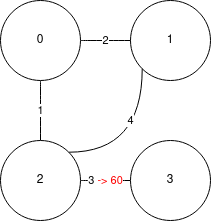
\includegraphics{upload_5c973d56c94fbd7d0646bba45e545d7c.png}

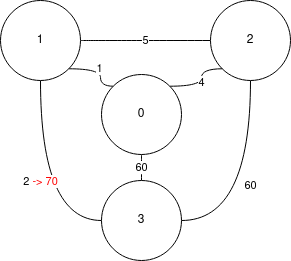
\includegraphics{upload_97a25790f5b60891fe1985f10196c3b7.png}

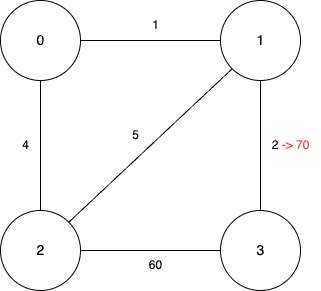
\includegraphics{upload_c90a572c0f84e1b171cf1dd6aac089d3.png}

view Distance-Vector Algorithm: Adding Poisoned Reverse in the text book

\url{https://en.wikipedia.org/wiki/Split\_horizon\_route\_advertisement}

\chapter{A solution to this problem}

Poison reverse doesn't solve all the count-to-infinity problems, we saw
in the previous problems that the problems still happen in some cases.
We can use route poisoning split horizon route advertisement to inform
all nodes that our distance to a node has changed. This means that we
have to find a way to broadcast this kind of message in our protocol.

\url{https://en.wikipedia.org/wiki/Split\_horizon\_route\_advertisement}

The RIP protocol uses a special kind of timer, when a routing cost is
increased, the timer is started and doesn't allow any modification and
will set the cost to infinity of the routing entry until it is finished.
Then the router can restart to compute the route. The timer is usefull
to wait for all the network to be aware of the cost increase. This timer
is called Holddown timer.

\url{https://en.wikipedia.org/wiki/Distance-vector\_routing\_protocol\#Count\_to\_infinity\_problem}

\url{https://en.wikipedia.org/wiki/Routing\_Information\_Protocol\#Timers}

\url{http://www.routeralley.com/guides/rip.pdf}

\chapter{Screenshot of the simulator running}

\section{3 node network}

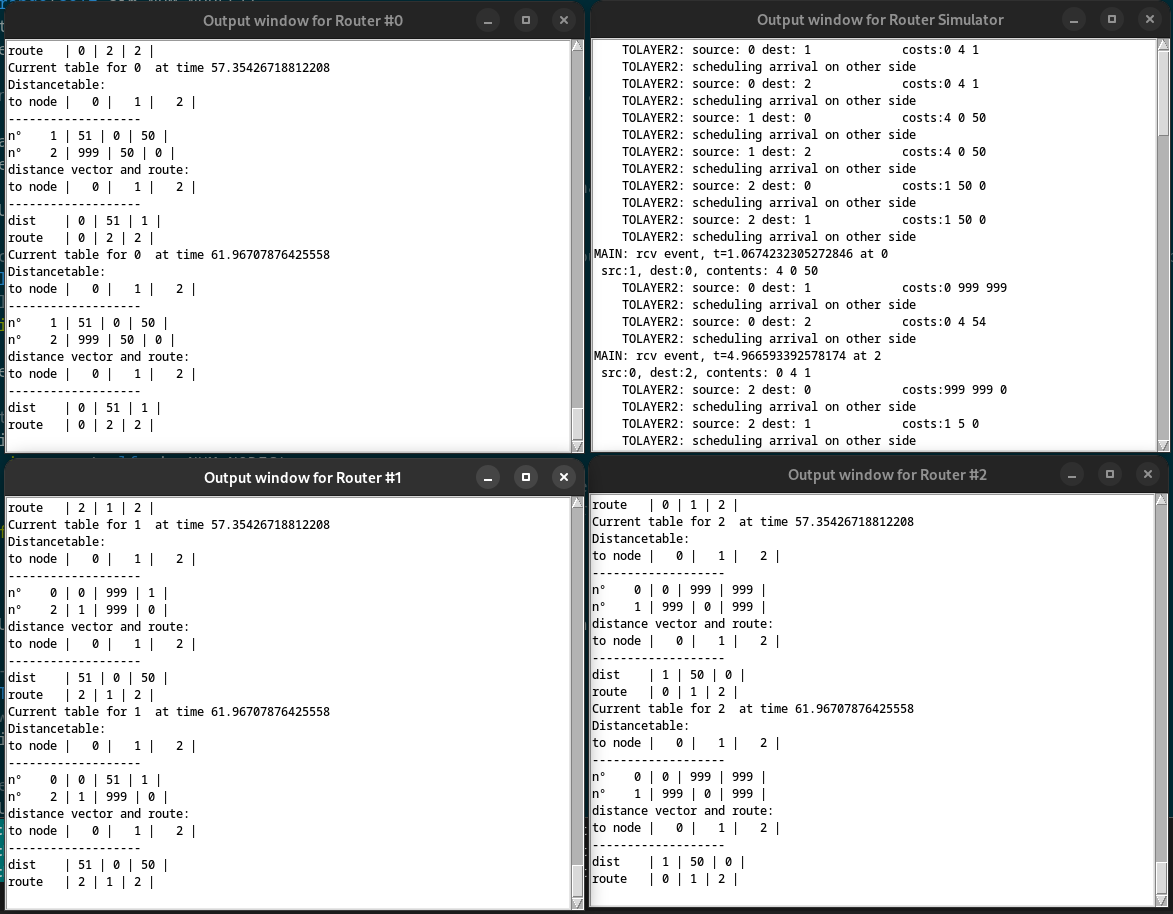
\includegraphics[width=\linewidth]{upload_f79f336d7f2818a70e34477d37d6e236.png}

\section{4 node network}

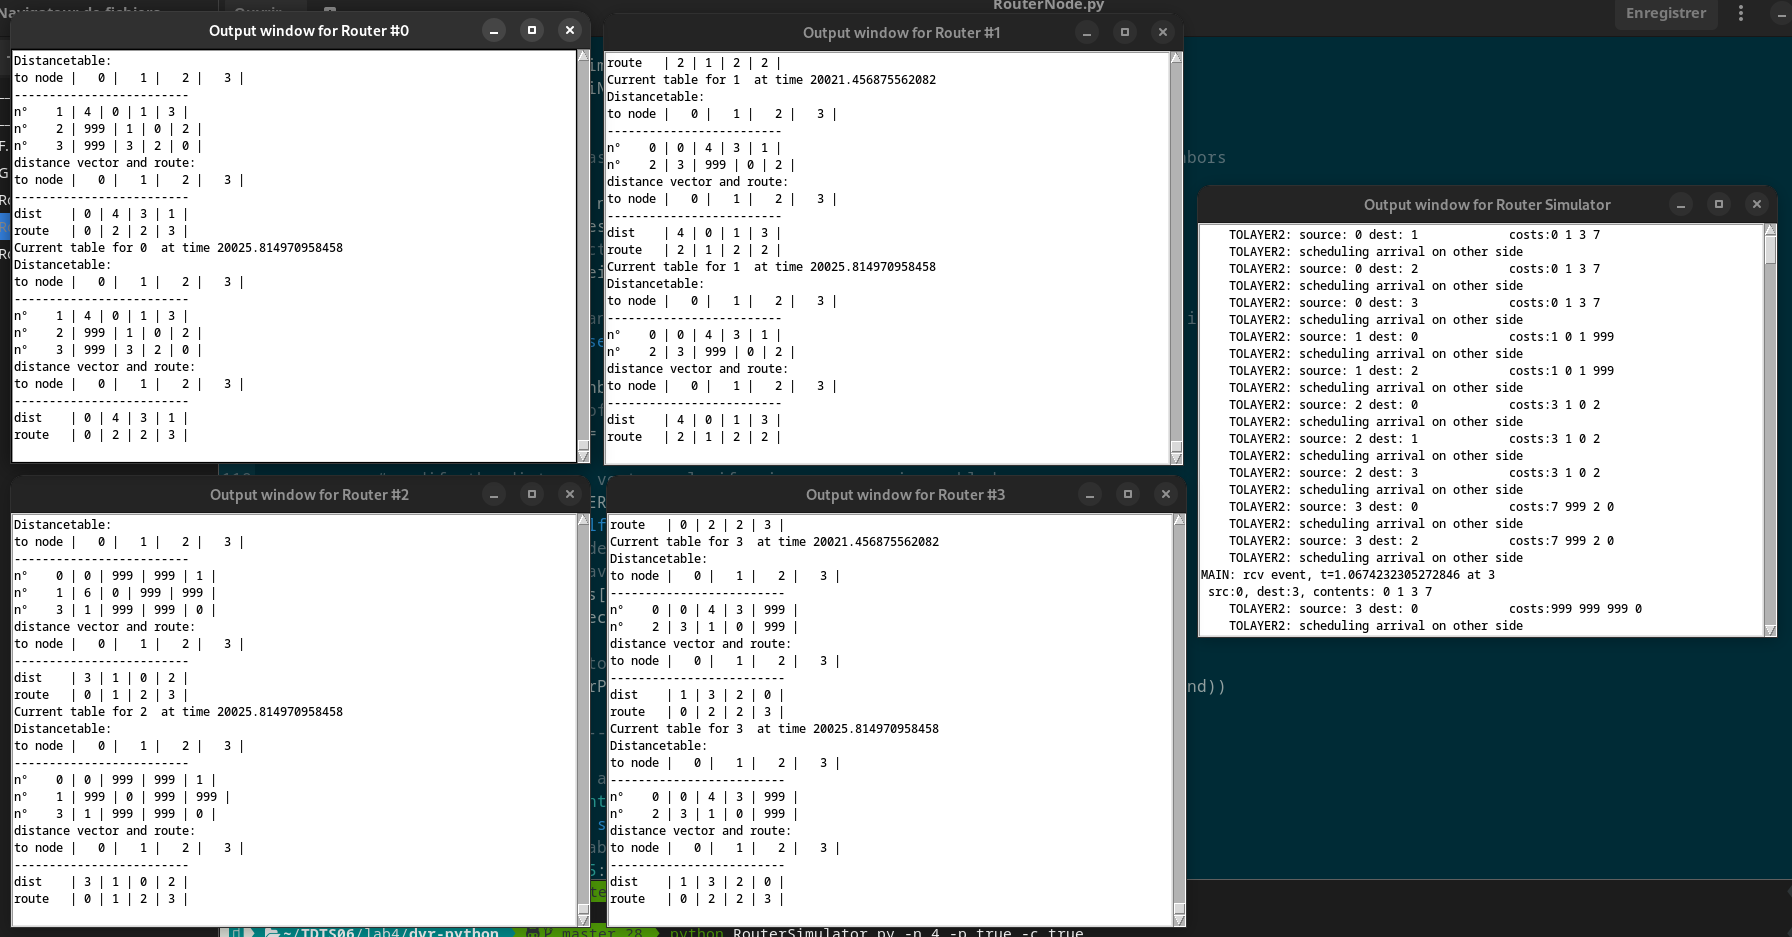
\includegraphics[width=\linewidth]{upload_9c613d09dbd091ad941cf9237feb2efd.png}

\section{5 node network}

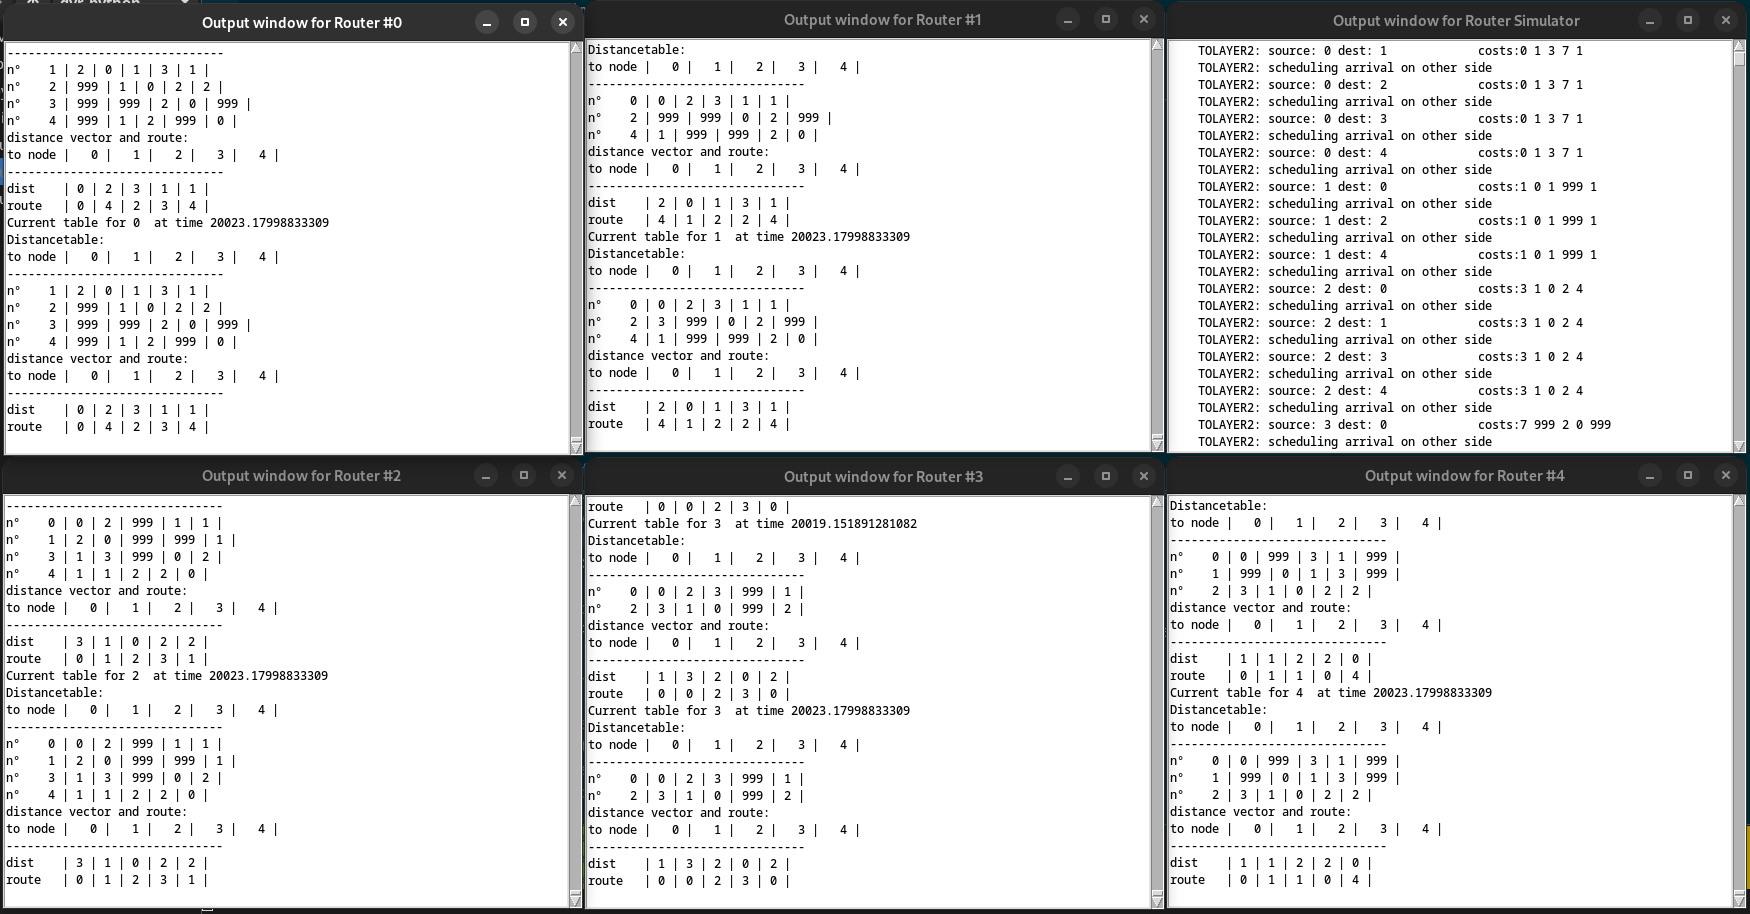
\includegraphics[width=\linewidth]{upload_1e6ba73192c8a539ba86155485f419e3.png}
\end{document}
